\documentclass[letterpaper]{article}
\usepackage{graphicx} % Required for inserting images
\usepackage{authblk}
%configure print geometry
\usepackage[margin=1.2in]{geometry}
\setlength{\parskip}{0.3\baselineskip}
% preferred reference package
\usepackage[style=numeric, sorting=none]{biblatex}
\addbibresource{refs.bib}

\title{An Engaging Approach to STEM Education: Case Studies from Video Game Glitches}
\author[1]{Jon Craton}
\affil[1]{Anderson University, Anderson, IN}
\date{} % no date, we will add it to the final version in the header

\begin{document}

\maketitle

\begin{abstract}
This work explores using classic video game glitches as case studies to demonstrate key concepts in computer science and cybersecurity. An example case from one of the most popular glitches found in Pokémon is explored. The case is evaluated as a learning instrument in an undergraduate computer science class and received positive qualitative feedback from students.
\end{abstract}

\section{Introduction}
Teaching in a manner that is both authentic and engaging is one of the persistent challenges for educators. While it would be ideal for all students to arrive at a learning experience intrinsically motivated, this is often not the case. While it is possible to compel students into educational activities through grades or the threat of a quiz, finding ways to encourage intrinsic motivation is more beneficial \cite{deci2013intrinsic}.

As educators, we can be tempted to rely heavily on direct instruction. This approach allows for relatively simple planning and execution, making a teacher out of anyone who can read text from a slide deck. However, a large body of research demonstrates that this approach is not best for learners. Active learning enhances student performance in STEM fields \cite{freeman2014active} and helps to close achievement gaps for underrepresented students \cite{theobald2020active}.

Case studies are a common educational tool. They allow students to explore and apply concepts to real-world situations. They have been shown to be valuable in computer science education because they can better capture the multi-dimensional decisions necessary to construct a correct and effective computer program \cite{linn1992case}.

A glitch is an unintended game behavior caused by bugs or unexpected system interactions that produces results different from the game's intended rules. This paper provides an outline for a video game glitch case study used in a classroom to enhance learning and encourage students in active exploration. Video game glitches are inherently engaging to many learners. It has been noted that some people who play video games enjoy video game glitches: ``one of the many ways in which a player may enjoy a video game is to explore it in search of these discrepancies, relishing the variety of effects they can cause'' \cite{bainbridge2007creative}.

\section{Theoretical Foundation}
Including live demonstrations in teaching can be intimidating for educators, especially if the demonstrations require skill and can fail in various ways for technical reasons. A lecture has very few failure modes, whereas more complex learning experiences can encounter various challenges. The benefits of taking this risk are well-documented. As Ken Bain notes, ``The best teaching is often both an intellectual creation and a performing art. It is both Rembrandt’s brush strokes and the genius of insight, perspective, originality, comprehension, and empathy that makes a Dutch Master'' \cite{bain2004best}.

For teaching to be genuinely engaging for students, it is important for it to be genuinely exciting for the teacher. As Parker Palmer notes, ``As I teach I project the condition of my soul onto my students, my subject, and our way of being together'' \cite{palmer2000courage}. Finding ways to add real exploration and excitement to teaching is valuable for both teachers and learners.

Part of good teaching is creating learning experiences that allow students to become open to a state where the deepest forms of knowledge acquisition can occur. It is not sufficient for students to listen and take notes; they must at times be truly confused and confront their ignorance with humility. This state has been described by Csikszentmihalyi in various ways, including ``what a painter feels when the colors on the canvas begin to set up a magnetic tension with each other, and a new thing, a living form, takes shape in front of the astonished creator'' \cite{csikszentmihalyi1990flow}.

Students are not merely learning static concepts that can be conveyed as facts from one person to another. Situated learning reminds us that a concept ``will continually evolve with each new occasion of use, because new situations, negotiations, and activities inevitably recast it in a new, more densely textured form'' \cite{brown1989situated}. In computer science, it has been suggested that encouraging more ``legitimate peripheral participation'' as described in situated learning can increase engagement and learning \cite{ben2004situated} \cite{guzdial2006imagineering}.

While it has been established that game-based learning can have a positive impact on learning, especially on younger learners \cite{arztmann2023effects}, the approach proposed here does not follow this pattern. The learning experience itself is not gamified. A game is simply used as an example case that can be deeply engaged by the intellectual challenge of debugging a complex, real-world system.

Kolb identified that true learning happens when we encounter a new experience, reflect on it, develop an abstract conceptualization, and engage in active experimentation \cite{kolb84}. Glitches in classic games provide an ideal platform to craft this learning cycle. An initial exploration brings with it a moment of confusion as assumptions about the simulated world are violated. This is followed by additional observation of the world that allows learners to construct a more accurate model of what is really happening behind the scenes. Finally, learners can test assumptions about their understanding through further experimentation in the world.

\section{Methodology for Classroom Demonstration}

The learning experience driven by this glitch case study is situated within a larger session on exceptions. The intended learning outcome from exploring the case is for students to be able to describe the importance of proper handling of exceptional cases to maintain the intended program state.

Exploring an in-game glitch first requires a mechanism that allows the glitch to be demonstrated and explored live in a classroom setting. This can be done by connecting a classic console to the classroom projection system, but this creates a number of challenges. It is tedious to transport and connect the system, and it also has limited ability to inspect and debug running games. For these reasons, it is often best to use some form of emulation. For this exploration, the open source higan\cite{ginder2004higan}  emulator was used.

In order to run a game under emulation, it is necessary to create an image of the read-only memory found on a game cartridge. There are various hardware tools and methods such as cartreader\cite{sanni_cartreader} or RetroBlaster\cite{retroblaster} to accomplish this. Once the ROM contents have been extracted, they can be stored for later use. Specialized hardware is not required in the classroom during emulation.

One desirable aspect of emulation technology is the ability to pause, slow down, or rewind time. Many game glitches require time consuming setup or precise execution, and having the ability to retry an attempt or quickly experiment with alternative approaches in response to live student feedback is desirable. Many emulation systems provide the ability to create and restore the entire state of a system at a given moment. This feature can be used to rapidly jump to a desired point within a game that would otherwise consume significant class time to discover.

\section{Glitch Case Study}
Pokémon Red is a 90s role-playing game for the Nintendo Game Boy where players explore the game world to capture and train creatures (Pokémon) and battle other trainers. The game launched a much larger franchise of related games, so while the game is now decades old, it remains a classic, and its formula will be familiar to many modern players. Its simple cartridge-based implementation and direct memory management led to well-known, exploitable glitches.

The case explored in this paper involves a well-known glitch colloquially referred to as the ``Old man glitch''. It is well understood and its underlying mechanics have already been described \cite{bulbapedia2005} \cite{scrumpy2016missing}. In fact, this glitch has even been used within computer science courses \cite{rjwalls2022}.

In order for students to appreciate the brokenness of the world, it is important for them to first see a glimpse of it as it was intended to be. We explore the correctly functioning world together, being sure to encounter each interaction that we will later see break down. This allows students who may have never encountered this game, or even similar games, to become oriented to the correctly functioning game world. We can then begin the setup necessary to trigger the glitched behavior.

This glitch causes the system to access and use memory that has not been properly initialized. In particular, it requires the player character in the game to engage in a wild Pokémon battle when the wild Pokémon data is not properly initialized. This allows the player to encounter and capture invalid or ``glitch'' Pokémon as shown below:

\begin{figure}[h!]
    \centering
    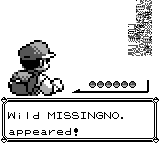
\includegraphics[width=0.4\textwidth]{missingno.png}
    \caption{Engagement with MissingNo glitch Pokémon}
\end{figure}

As the player character navigates the virtual world, they have opportunities to discover and battle wild Pokémon. The Pokémon faced are drawn from a list that is populated by game region, so that players are presented with access to new varieties as they progress through areas of the game.

At one point in the game, the player is taught how to catch Pokémon by a character known simply as ``Old Man''. In order to demonstrate catching Pokémon, the game scripts what would normally be player actions in order to demo catching a Pokémon as a cutscene. A naive approach to this would leave the player's name as the one engaging in the encounter, so the player's name must be temporarily replaced by ``Old Man'' in memory. The software later needs to restore the player's correct name, so it must be stored elsewhere temporarily. The memory location used for temporary storage happens to be the location for some wild Pokémon encounter data, as it is not needed in the region where ``Old Man'' is found.

\begin{table}[h!]
\centering
\begin{tabular}{cll}
Address &              Purpose &   Value \\
   d887 & Grass Encounter Rate & name[0] \\
   d888 &              Level 1 & name[1] \\
   d889 &            Pokémon 1 & name[2] \\
   d88a &              Level 2 & name[3] \\
   d88b &            Pokémon 2 & name[4] \\
   d88c &              Level 3 & name[5] \\
   d88d &            Pokémon 3 & name[6] \\
   d88e &              Level 4 &    0x80 \\
   d88f &            Pokémon 4 &    0x00 \\
\end{tabular}
\caption{Pokémon encounter table values overwritten by player's name}
\end{table}

After the demonstration cutscene, the player's name is restored, but the wild Pokémon encounter data is left in an invalid, uninitialized state. While this data is accessible, the player's name was certainly never meant to be treated as wild Pokémon encounters. This data is not needed in the current region, and it is re-initialized as the player moves regions, so it does not generally cause an issue. However, if the player can move to a region that does not re-initialize this part of the wild Pokémon encounter data and trigger an appropriate wild Pokémon encounter, improperly initialized data will be used to select a Pokémon for the encounter. This can be exploited by immediately flying to Cinnabar Island.

Cinnabar Island was not intended to include wild Pokémon encounters, so it does not re-initialize the wild Pokémon data. Data from the previous region, or in this case improperly initialized data, would be used for any encounters. Due to a separate bug, one small strip of water to the east of Cinnabar Island does allow encounters, and these will trigger the glitch.

\begin{figure}[h!]
    \centering
    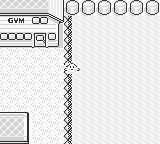
\includegraphics[width=0.4\textwidth]{surfing.png}
    \caption{Triggering an engagement near Cinnabar Island}
\end{figure}

This glitch study provides numerous opportunities for learning. A real interactive example like this is multifaceted and can be explored in real time. There are several issues that work together to allow the final issue, showing the importance of defense in depth (the idea that multiple, overlapping security controls reduce risk because if one control fails, others still protect the system). In this case, minor flaws in different areas combined to produce the observable glitch, showing why relying on a single safeguard can be insufficient and why layered protections and redundant checks are valuable.

From a cybersecurity standpoint, it can be valuable to consider the root cause of this issue. Perhaps it could be mapped to an appropriate framework, such as identifying the cause as ``Use of Uninitialized Resources'' (CWE-908) \cite{mitre2012}. From there, learners can discuss and explore potential mitigations for this sort of software weakness.

The instructor can pose a number of guiding questions to help drive discussion in the intended direction:

\begin{itemize}
    \item What assumptions in the original code are violated by this interaction?
    \item What boundary checks, validation, or safer memory management practices could have prevented this glitch?
    \item What trade-offs would mitigations incur?
    \item In Python, what exceptions would you expect if code attempted to use an unexpected value?
    \item How would catching these exceptions prevent crashes or corrupted state?
\end{itemize}

It is possible to take this example farther if desired. For example, what happens when we catch one of these glitch Pokémon? Do these encounters have any impact on the rest of the game? In Pokémon, the player character has an inventory of items that are used to complete quests or provide benefits throughout the game. There are also memory locations used to store data about which Pokémon have been seen and caught. As it turns out, encounters with glitch Pokémon trigger an invalid write, due to their unexpected IDs, and cause the quantity of the sixth item in a player's inventory to be set to 128 \cite{bulbapedia2010}. This can be used to demonstrate how seemingly benign software issues can sometimes be exploited to gain elevated privileges in unexpected ways.

\section{Assessment}
This case study was situated within a larger 50-minute learning session covering the value of proper exception handling. At the start of the session, students were given the opportunity to take a short multiple choice quiz testing knowledge of this concept. Following the session, students were allowed to retake the same assessment. This quiz included three multiple questions allowing students to demonstrate that they understood the key points from the session.

An analysis of the quiz results showed that the paired differences contained multiple ties and deviated from normality, so a Wilcoxon signed-rank test was conducted to examine whether post-test scores were greater than pre-test scores for the nine participants. The mean difference was 22.22 (SD = 28.87). The Wilcoxon signed-rank test indicated a non-significant trend toward higher post-test scores, W = 10.00, p = .063 (one-tailed). A paired-samples t-test indicated a statistically significant increase in scores from the pre-test (M=70.3,SD=30.9) to the post-test (M=92.5,SD=14.7), with a p-value of p=0.049, but this result should be interpreted with caution due to violation of the t‑test normality assumption.

Qualitatively, students reported being more actively connected to their learning experience via the case study. One student called it ``very engaging'', and another referred to it as being ``much better than usual teaching''.

This assessment is admittedly limited. It measures the impact of a single case in a single relatively small classroom, but it does demonstrate that there may be potential to this type of case study tool as a way to enhance student engagement and learning. The positive qualitative feedback suggests that this method holds promise for enhancing student engagement and learning.

\section{Discussion and Future Work}

The idea of video game glitches as case studies of software engineering, computer science, and cybersecurity is compelling for many students. It allows them to connect experiences from their lives with content from the classroom and provides a mechanism for situating classroom knowledge within real software systems.

Video games provide a very natural presentation for software concepts. By their nature, they are not merely visible but also often flashy and attention grabbing. By violating the rules of simulated environments, educators can create a moment of confusion and delight that captures attention and provides a platform for diagnosing and exploiting complex software issues.

While this study is limited in scope and explores only a single case in a single classroom, this work could be significantly expanded in the future. Additional cases could be crafted and shared for use in a broader set of classrooms. Cases could also be evaluated more rigorously and broadly by expanding studies to additional classrooms and comparing this case study approach against other teaching methods that have similar aims.

%\bibliographystyle{plain}
%\bibliography{refs}

\printbibliography
\end{document}